\documentclass[12pt]{article} % article class, 12pt font

% load any packages you need for more custom stuff
\usepackage[margin=1in]{geometry} % set 1-inch margins
\usepackage{setspace}\doublespacing % set double spacing
\usepackage[superscript]{cite} % superscript numeric in-line citations
\usepackage{indentfirst} % indent the first paragraph of each section
\usepackage{graphicx} % enable displaying png format graphs
\usepackage{csvsimple} % enable importing tabular data
\usepackage{booktabs} % enable formulating tables


% set title stuff
\title{Sample Document}
\newcommand{\authors}{Hans de Moor}
\author{Math 114 Mathematical Modeling\\St. Mary's College}
\date{February 13, 2019}

% start the actual document
\begin{document}

% create title stuff
\hfill\authors % write the authors right-aligned
%\vspace{-0.5in} % reduce space before title
{\let\newpage\relax\maketitle} % print title

% begin the main text
\section*{Preface}
This sample document illustrates suggestions for making homework and project reports. The content of this example is based on Example 2, Mortgaging a Home, in Section 1.1 of the adopted text for this course. In addition to showing some of the style and format suggestions, examples are given of how to show equations, import and display tabular data and displaying graphs. A companion document is available that gives sample code written in Python to be used with Spyder to compute, organize and graph the data in the example.

\section*{Problem Statement}
A home was purchased by financing \$80,000 for 20 years, paying a monthly payment of \$880.87 with a monthly rate of 1\%. They have made 72 payments and wish to know how much they owe on the mortgage. They wish to consider paying off the mortgage or refinancing with different interest rates.

\section*{Method}

The change in the amount owed each period increases by the amount of interest on the balance due and decreases by the monthly payment.

$\Delta b_n = b_{n+1} - b_n = 0.01 b_n - 880.87$

Solving for $b_{n+1}$ yields the dynamical model

$b_{n+1} = b_n + 0.01 b_n - 880.87$

A table can be made of the monthly balances.

\section*{Results}
\begin{center}
\csvautobooktabular[table head=\toprule\bfseries Month & \bfseries Balance\\\midrule\csvlinetotablerow\\]{homemortgage.csv}
 

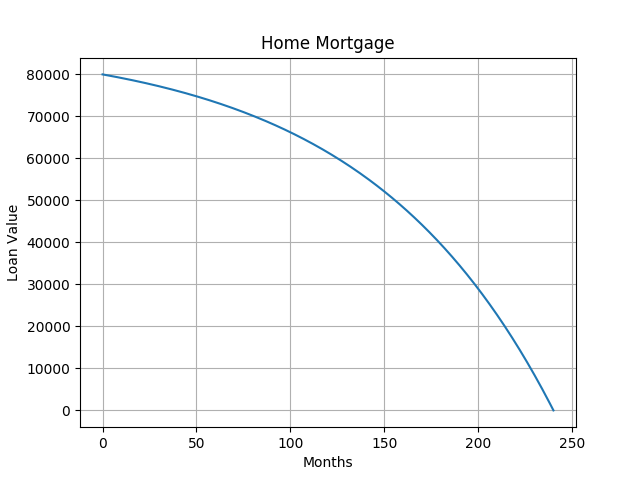
\includegraphics{homemortgage.png}
\end{center}

\section*{Discussion}
 The discussion section should be used to address issues such as variability, various options to consider, sensitivity to assumptions and any other consideration in addressing the problem.
 
\section*{Conclusions}
The conclusion should address the solutions to the problem in a straight forward fashion. The results should be in terms that the one posing the question can understand. Frequently questions requiring a model are stated in non-technical terms, and so the answer should stated in a way that the person posing the question can understand.

\end{document} % this ends your document